%!TEX encoding = UTF-8 Unicode%
% Este es el trabajo de Gabinete expedido el Mayo de 2010.
% Tema: CMOS Setup
% Integrantes:
%	* Kenny Meyer
%	* Ana Benitez
%	* Maria Monsserat Silva
%	* Fabiola Ruiz Leiva
\documentclass[12pt,oneside,a4paper]{article}
\usepackage{style}
\begin{document}
\title{CMOS Setup}
\author{Ana Benitez (\texttt{ana\_benitez\_py@hotmail.com}), \\
		Maria Monserrat Silva (\texttt{monse\_14\_fob@hotmail.es}), \\
		Fabiola Ruiz Leiva (\texttt{fabiola.ruiz.leiva@gmail.com}), \\ 
		Kenny Meyer (\texttt{knny.myer@gmail.com})}
\date{Mayo 2010}
\maketitle
\clearpage

% Factores que tener en cuenta:
%  * La documentacion sera leida por los companeros
%  * Tiene que ser comprensiva y completa.
%

% The basic structure of the project:
% 
\setcounter{tocdepth}{3}
\tableofcontents
\newpage

\section{Introducción}\label{sec:introduccion}

Cuando encendemos la computadora, el sistema operativo se encuentra o bien, en
el disco duro o bien en un disquete; sin embargo, si se supone que es el
sistema operativo el que debe dar soporte para estos dispositivos, {\em ¿cómo podría
hacerlo si aún no está cargado en memoria?}

Lo que es más:
\begin{itemize}
	\item ¿Cómo sabe la computadora que tiene un disco duro (o varios)?
	\item ¿Y la disquetera?  
	\item ¿Cómo y dónde guarda esos datos, junto con el tipo de memoria y cache?
	\item ¿O algo tan sencillo pero importante como la fecha y la hora? 
\end{itemize}

Por ende, la unidad y programa que se encarga de todo esto es la BIOS.
Resulta evidente que la BIOS debe poderse modificar para alterar estos datos
(al añadir un disco duro o cambiar al horario de verano, por ejemplo); por ello
las BIOS se implementan en memoria. \\
Pero además debe mantenerse cuando apaguemos nuestra pc, porque no tendría
sentido tener que introducir todos los datos en cada arranque; por eso se usan
memorias especiales, que no se borran al apagar el ordenador: memorias tipo
CMOS (no volatil), por lo que muchas veces el programa que modifica la BIOS se
denomina {\bf CMOS Setup}.

\newpage

\section{Conceptos}\label{sec:conceptos}

	\subsection{La RAM}{\label{sec:conceptos/RAM}}

		La memoría de acceso aleatorio (en {\bfseries inglés Random Access Memory} cuyo
		acrónimo es {\bfseries RAM}) es la memoría donde el procesador recibe las
		instrucciones y guarda los resultados. Es el área de trabajo paara la mayor
		parte del software de un computador.

	\subsection{La ROM}{\label{sec:conceptorom}}

		Memoría de solo lectura ({\bfseries Read-only memory}) es una
		clase de medio de almacenamiento usado en los ordenadores y otros dispositivos
		electrónicos. Los
		datos en la ROM no se pueden modificar al menos no de una manera rápida o fácil
		y se usa principalmente para contener el Firmware.

	\subsection{El Firmware}{\label{sec:conceptos/firmware}}

		Firmware o programación en firme, es un bloque de instrucciones de
		programa para propositos específicos grabada en una memoría de tipo no volátil
		( ROM, EPROM, Flash, ...) que establece la lógica de más bajo nivel que
		controla los circuitos electrónicos de un dispositivo de cualquier tipo.

	\subsection{El CMOS}{\label{sec:conceptos/CMOS}}

		{\bf CMOS} es la contracción de {\em Complementary Metal Oxide Semiconductor}, o
		Tecnología Metal Óxido Semiconductor Complementario. \\
		Es una tecnología utilizada para fabricar circuitos integrados (chips), que
		para el caso es un memoria del tipo ROM, en la actualidad FLASH ROM (se
		borran electricamente) donde se guarda información básica del equipo como el
		BIOS y el SETUP. \\ 
		{\bf Esta memoria tiene una porción que funciona como RAM, donde se guarda la
		configuración que el usuario le da al equipo y algunas configuraciones
		establecidas de fábrica.} \\ 
		Otra información que se guarda en el y que se accede mediante el SETUP
		es la fecha y la hora del sistema, y para que la misma se mantenga
		actualizada debe estar siempre alimentada, es por esto que en toda
		computadora encontraremos una pila para alimentar dicho circuito.

		\subsubsection{El RAM-CMOS}\label{sub:el ram-cmos}

			RAM-CMOS es un tipo de memoria en que se guardan los datos que se
			pueden configurar del BIOS y contiene información básica sobre algunos
			recursos del sistema que son susceptibles de ser modificados como el
			disco duro, el tipo de disco flexible, etc. \\
			Esta información es almacenada en una RAM, de 64 bytes de capacidad,
			con tecnología CMOS, que le proporciona el bajo consumo necesario para
			ser alimentada por una pila que se encuentra en la placa base y que
			debe durar años, al ser necesario que este alimentada constantemente,
			incluso cuando el ordenador se encuentra apagado. Para ello
			antiguamente se usaba una batería recargable que se cargaba cuando el
			ordenador se encendía. \\
			Mas modernamente se ha sustituido por una pila desechable de litio
			(generalmente modelo CR-2032) y que dura de 2 a 5 años.

	\subsection{El BIOS}{\label{sec:conceptobios}}

		BIOS es la contracción de Basic Input Output System, o Sistema Básico de
		Entrada – Salida. \\
		Es un programa muy básico, normalmente programado en lenguaje ensamblador,
		cuya misión es la de arrancar o posibilitar el ``Booteo'' de la computadora.
		A pesar de tratarse de un programa sumamente básico resulta totalmente
		indispensable, ya que sin el BIOS sería imposible que una computadora pudiera
		iniciar.

	\subsection{CMOS Setup}\label{sub:cmos setup}
	
		Basicamente el CMOS Setup es el programa que puede modificar todos los parametros
		guardada en la CMOS de forma visual y tangible (con el teclado). \\
		El CMOS Setup es una serie de instrucciones generalmente escrito en
		lenguaje Ensemblador que se lee de la BIOS al arrancar la computadora. \\
		Se suelen usar los terminos CMOS Setup y BIOS Setup como sinonimos para
		indicar lo mismo, pero son dos diferentes circuitos en la placa base. \\

	\subsection{LBA}\label{sec:lba}

		LBA (siglas de logical block addressing, dirección lógica de bloques)
		es un método muy común usado para especificar la localización de los
		bloques de datos en los sistemas de almacenamiento, principalmente
		secundario, del ordenador. El término LBA puede referirse también a la
		dirección del bloque al que enlaza.  Los bloques lógicos en los
		ordenadores modernos son normalmente de 512 o 1024 bytes cada uno.

	\newpage

\section{El proceso de inicio}\label{sec:arranque}

	%The system BIOS is what starts the computer running when you turn it on.
	%The following are the steps that a typical boot sequence involves. Of
	%course this will vary by the manufacturer of your hardware, BIOS, etc., and
	%especially by what peripherals you have in the PC. Here is what generally
	%happens when you turn on your system power:

	\begin{enumerate}
		\item[1]El sistema BIOS es lo que inicia la computadora cuando la
			encendemos.  Los siguientes pasos son los pasos que involucra la
			secuencia de booteo típico.  Por supuesto esto depende del
			fabricante de la hardware, BIOS, etc., y especialmente por los
			perífericos de la PC. Esto es lo que pasa por lo general cuando
			encendemos la energía de la computadora.

	%The internal power supply turns on and initializes. The power supply takes
	%some time until it can generate reliable power for the rest of the
	%computer, and having it turn on prematurely could potentially lead to
	%damage. Therefore, the chipset will generate a reset signal to the
	%processor (the same as if you held the reset button down for a while on
	%your case) until it receives the Power Good signal from the power supply.
	
		\item[2] La fuente de alimentación interna se enciende y se inicializa.
			La fuente de alimentación necesita algún tiempo para generar
			energía seguro para el resto de la computadora, y enciendola antes
			de tiempo potencialmente puede causar daños. Por lo tanto el
			chipset va a enviar una señal de reseteo al procesador (es lo mismo
			que como si uno fuera apretando el botón de RESET) hasta que recibe
			el ``Power Good'' señal de la fuente de alimentación.

	%When the reset button is released, the processor will be ready to start
	%executing. When the processor first starts up, it is suffering from
	%amnesia; there is nothing at all in the memory to execute.  Of course
	%processor makers know this will happen, so they pre-program the processor
	%to always look at the same place in the system BIOS ROM for the start of
	%the BIOS boot program. This is normally location FFFF0h, right at the end
	%of the system memory. They put it there so that the size of the ROM can be
	%changed without creating compatibility problems. Since there are only 16
	%bytes left from there to the end of conventional memory, this location just
	%contains a "jump" instruction telling the processor where to go to find the
	%real BIOS startup program.  
	
		\item[3] Cuando el botón de resteo es liberado, el procesador va a
			estar listo para ejecutar acciones.  Al inidcio el procesador no
			trabaja nada; no hay nada en la memoría para ser procesado.  Por lo
			tanto se carga instrucciones de la BIOS\ref{sec:conceptobios}
			ROM\ref{sec:conceptorom}, normalmente en la posición de la memoría
			FFFF0h, los últimos de 16 bits de la memoría, donde está guardada
			la posición del programa del BIOS booteo o bien POST(Auto
			diagnóstico al encender) para ser procesadas.

	%The BIOS performs the power-on self test (POST). If there are
	%any fatal errors, the boot process stops. POST beep codes can be found in this
	%area of the Troubleshooting Expert.
	
		\item[4] El BIOS realiza el POST(Auto diagnóstico al encebuiltinnder). Si hay une
			error fatal, el proceso de inicio se detiene. Errores son desplegadas
			por una secuencia de pítidos con significados concretos.
	
	%The BIOS looks for the video card. In particular, it looks for the video
	%card's built in BIOS program and runs it.  This BIOS is normally found at
	%location C000h in memory. The system BIOS executes the video card BIOS,
	%which initializes the video card. Most modern cards will display
	%information on the screen about the video card. (This is why on a modern PC
	%you usually see something on the screen about the video card before you see
	%the messages from the system BIOS itself).  The BIOS then looks for other
	%devices' ROMs to see if any of them have BIOSes. Normally, the IDE/ATA hard
	%disk BIOS will be found at C8000h and executed. If any other device BIOSes
	%are found, they are executed as well.  

		\item[5] El BIOS busca la tarjeta de video. En particular, busca el
			Firmware de la tarjeta de video y lo ejecuta. Este firmware
			generalmente se encuentra en la posicion de memoria C000h.  El
			sistema BIOS ejecuta el Firmware de la tarjeta de video, lo cual
			inicializa la tarjeta. La mayoria de las tarjetas de video modernas
			van a desplegar informacion en pantalla acerca de la tarjeta de
			video. (Esta es la razon, por la cual ves mensajes en la pantalla
			al inciar la computadora) El BIOS entonces busca los Firmwares de
			otros dispositivos para ver si estos tienen BIOSes.
				
	%The BIOS displays its
	%startup screen.  
		\item[6] El BIOS muestra la pantalla inicial.
			\begin{figure}[H]
				\centering
					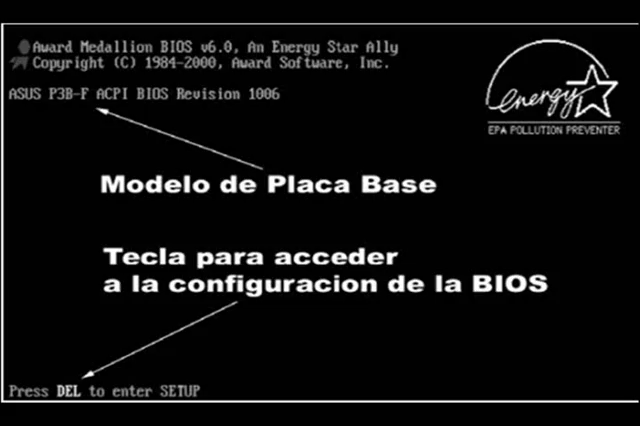
\includegraphics[scale=0.3]{img/Screenshot-Ingresando_al_BIOS_Setup-1.png}
				\caption{El BIOS al encender la computadora.}
			\end{figure}
	
    %The BIOS does more tests on the system, including the memory
	%count-up test which you see on the screen. The BIOS will generally display a
	%text error message on the screen if it encounters an error at this point; these
	%error messages and their explanations can be found in this part of the
	%Troubleshooting Expert.  

	\item[6] El BIOS hace mas pruebas del sistema, incluyendo el conteo de memoria
		RAM. \\
		Generalmente ahora si ocurren errores fatales se los desplegara en la
		pantalla en vez de una notificación auditiva.

	%The BIOS performs a "system inventory" of sorts, doing
	%more tests to determine what sort of hardware is in the system. Modern BIOSes
	%have many automatic settings and will determine memory timing (for example)
	%based on what kind of memory it finds. Many BIOSes can also dynamically set
	%hard drive parameters and access modes, and will determine these at roughly
	%this time. Some will display a message on the screen for each drive they detect
	%and configure this way. The BIOS will also now search for and label logical
	%devices (COM and LPT ports).  

	%If the BIOS supports the Plug and Play standard,
	%it will detect and configure Plug and Play devices at this time and display a
	%message on the screen for each one it finds. See here for more details on how
	%PnP detects devices and assigns resources.  
	\item[7] El BIOS ahora realiza un sistema de inventario de sorteos, haciendo
		más pruebas para determinar el tipo de hardware del sistema.
		BIOSes modernos tienen ajustes automáticos y determinarán la sincronización
		de la memoría (por ejemplo) basado en que tipo de memoría de encuentra.
		Muchos BIOSes tambien pueden determinar {\em automáticamente} parametros
		del disco duro y los modos de acceso, y determinará estos aproximadamente
		en este período.
		Algunas desplegarán un mensaje en la pantalla para cada unidad/dispositivo que
		se detecta y lo configura a esa manera. El BIOS ahora buscará y calificará los
		dispositivos lógicos. \\*
		Si el BIOS soporta el estándar {\emph Plug-and-Play }\cite{plugandplay} este detectará
		y configurará los dispositivos {\emph Plug-and-Play} mientras y mostrará un mensaje
		en pantalla para cada dispositivo registrado.
	
	%The BIOS will display a summary
	%screen about your system's configuration. Checking this page of data can be
	%helpful in diagnosing setup problems, although it can be hard to see because
	%sometimes it flashes on the screen very quickly before scrolling off the top.

	\item[8] El BIOS mostrará un resumen en pantalla de la configuración del sistema.  Revisando
		esta página puede ayudar en diágnosticar problemas con la configuración, a
		pesar de que lo puede resultar díficil porque se despide muy rapidamente. \\
		{\bf Truco:} Apretar la tecla <PAUSE>.

	%The BIOS begins the search for a drive to boot from. Most modern BIOSes contain
	%a setting that controls if the system should first try to boot from the floppy
	%disk (A:) or first try the hard disk (C:). Some BIOSes will even let you boot
	%from your CD-ROM drive or other devices, depending on the boot sequence BIOS
	%setting.
	
	%Having identified its target boot drive, the BIOS looks for boot
	%information to start the operating system boot process. If it is searching a
	%hard disk, it looks for a master boot record at cylinder 0, head 0, sector 1
	%(the first sector on the disk); if it is searching a floppy disk, it looks at
	%the same address on the floppy disk for a volume boot sector.
	
	%If it finds what
	%it is looking for, the BIOS starts the process of booting the operating system,
	%using the information in the boot sector. At this point, the code in the boot
	%sector takes over from the BIOS. The DOS boot process is described in detail
	%here. If the first device that the system tries (floppy, hard disk, etc.) is
	%not found, the BIOS will then try the next device in the boot sequence, and
	%continue until it finds a bootable device.  
	
	%If no boot device at all can be
	%found, the system will normally display an error message and then freeze up the
	%system. What the error message is depends entirely on the BIOS, and can be
	%anything from the rather clear "No boot device available" to the very cryptic
	%"NO ROM BASIC - SYSTEM HALTED". This will also happen if you have a bootable
	%hard disk partition but forget to set it active.  
	
	%This process is called a
	%"cold boot" (since the machine was off, or cold, when it started). A "warm
	%boot" is the same thing except it occurs when the machine is rebooted using
	%{Ctrl}+{Alt}+{Delete} or similar. In this case the POST is skipped and the boot
	%process continues roughly at step 8 above.

	\item[9] La próxima tarea del BIOS consiste en buscar un sistema operativo
		la cual cargará en la memoría. Si la busqueda fue exitosa, el BIOS se despide
		y vemos normalmente la pantalla de carga del sistema operativo.

	\end{enumerate}
	\newpage

\section{El BIOS}{\label{sec:bios}}

	Es indispensable conocer el concepto y las funciones que cumple el BIOS antes de tratar el CMOS Setup.

	El concepto del BIOS:
	\begin{quotation}

		{\em BIOS es la contracción de Basic Input Output System, o Sistema Básico de
		Entrada – Salida. 
		Es un programa muy básico, normalmente programado en lenguaje ensamblador,
		cuya misión es la de arrancar o posibilitar el “Booteo” de la computadora.
		A pesar de tratarse de un programa sumamente básico resulta totalmente
		indispensable, ya que sin el BIOS sería imposible que una computadora pudiera
		iniciar.}

	\end{quotation}
			
	\subsection{Marcas de BIOS}\label{sub:marcas de bios}
		Para mencionar algunas:
		\begin{enumerate}
			\item Award
			\item Phoenix
			\item American Megatrends Inc. (AMI)
		\end{enumerate}
	
	\subsection{Tipos de BIOS}\label{sub:chips bios}
		
		\begin{description}
			\item[ROM] Sólo se puede grabar en el momento que se fabrica el
				chip. La información que contiene no se puede alterar.
			\item[EEPROM] Estos chips se pueden grabar con luz ultravioleta. En
				la parte superior del chip se puede apreciar una especie de
				ventanilla transparente, que suele estar tapada con una
				pegatina. Estas BIOS se encuentra principalmente en 286 y 386.
				\cite{EEPROM}
			\item[Flash BIOS] Son los más utilizados en la actualidad. Estos
				chips se pueden grabar mediante impulsos eléctricos por lo que
				el propietario del ordenador la puede actualizar con un
				programa.
		\end{description}

		\newpage
		%\subsection{Solución de problemas}{\label{sec:bios/solucion-de-problemas}}
			%\subsubsection{Pitidos de la BIOS (Award)}{\label{sec:bios/tonos-de-la-bios}}

			%En esta seccion cubriremos los significados de los pitidos de los BIOS {\em Award}. \\
			%En la mayoría de los pitidos se les acompaña un mensaje de error. 

				%\paragraph{Tono ininterrumpido}:
				
				%Fallo en el suministro elctrico. Revisamos las conexiones y la fuente
				%de alimentación.  Tonos cortos constantes: Sobrecarga elctrica, chips
				%defectuosos, placa mal.

				%\paragraph{1 largo}:

				%Si aparece esto en la pantalla “RAM Refresh Failure”, significa que los
				%diferentes componentes encargados del refresco de la memoria RAM fallan
				%o no están presentes. Cambiar de banco la memoria y comprobar los
				%jumpers de buses. 

				%\paragraph{1 largo y 1 corto}: 

				%El código de la BIOS esta corrupto o defectuoso, probaremos a flasear o
				%reemplazamos el chip de la BIOS sino podemos cambiamos de placa. 

				%\paragraph{1 largo y dos cortos}:
				
				%No da señal de imagen, se trata de que nuestra tarjeta de vídeo esta
				%estropeada, probaremos a pincharla en otro slot o probaremos otra
				%tarjeta gráfica. 

				%\paragraph{1 largo y 2 cortos}:

				%Si aparece por pantalla este mensaje: “No video card found”, este error
				%solo es aplicable a placas base con tarjetas de vídeo integradas. Fallo
				%en la tarjeta gráfica, probaremos a deshabilitarla y pincharemos una
				%nueva en cualquier slot libre o cambiaremos la placa madre. 

				%\paragraph{1 largo y 3 cortos}:

				%Si aparece este mensaje por pantalla “No monitor connected” Idem que el
				%anterior. 

				%\paragraph{1 largo y varios cortos}: 

				%Mensaje de error. “Video related failure”. Lo mismo que antes. Cada
				%fabricante implanta un código de error según el tipo de tarjeta de
				%video y los parámetros de cada BIOS.

				%\paragraph{2 largos y 1 corto}:
				
				%Fallo en la sincronización de las imágenes. Cargaremos por defecto los
				%valores de la BIOS e intentaremos reiniciar. Si persiste nuestra
				%tarjeta gráfica o placa madre están estropeadas. 

				%\paragraph{2 cortos}:
				
				%Vemos en la pantalla este error: “Parity Error”. Se trata de un error
				%en la configuración de la BIOS al no soportar la paridad de memoria, la
				%deshabilitamos en al BIOS. 

				%\paragraph{3 cortos}:
				
				%Vemos en la pantalla este error. Base 64 Kb “Memory Failure”, significa
				%que la BIOS al intentar leer los primeros 64Kbytes de memoria RAM
				%dieron error. Cambiamos la RAM instalada por otra. 

				%\paragraph{4 cortos}:
				
				%Mensaje de error; “Timer not operational”. El reloj de la propia placa
				%base esta estropeado, no hay más solución que cambiar la placa. No
				%confundir con “CMOS cheksum error” una cosa es la pila y otra el
				%contador o reloj de la placa base. 

				%\paragraph{5 cortos}:
				
				%Mensaje por pantalla ``Processor Error'' significa que la CPU ha generado
				%un error porque el procesador o la memoria de vídeo están bloqueados. 

				%\paragraph{6 cortos}:

				%Mensaje de error: ``8042 - Gate A20 Failure'', muy mítico este error.
				%El controlador o procesador del teclado (8042) puede estar en mal
				%estado. 
				%La BIOS no puede conmutar en modo protegido. Este error se
				%suele dar cuando se conecta/desconecta el teclado con el ordenador
				%encendido. 

				%\paragraph{7 cortos}:
				
				%Mensaje de error: “Processor Exception / Interrupt Error”
				%Descripción. La CPU ha generado una interrupción excepcional o
				%el modo virtual del procesador está activo. Procesador a punto
				%de morirse. 

				%\paragraph{8 cortos}:
				
				%Mensaje de error: ``Display Memory Read / Write error''. La tarjeta de video esta estropeada, procedemos a cambiarla. 

				%\paragraph{9 cortos}:
				
				%Mensaje de error: ``ROM Checksum Error''; el valor del checksum (conteo de la memoria) de la RA

			%\newpage

	\subsection{Errores en pantalla}\label{sub:errores en pantalla}
	
	Los siguientes errores de pantalla son errores generales o bien, no
	dependen de marca y modelo de la BIOS:

		\subsubsection{BIOS ROM checksum error – system halted}

		El código de control de la BIOS es incorrecto, lo que indica que puede
		estar corrupta. En caso de reiniciar y repetir el mensaje, tendremos
		que reemplazar al BIOS.

		\subsubsection{CMOS battery failed}

		La pila de la placa base que alimenta la memoria CMOS ha dejado de
		suministrar corriente. Es necesario cambiar la pila inmediatamente.

		\subsubsection{CMOS checksum error – Defaults loaded}

		El código de control de la CMOS no es correcto, por lo que se
		procede a cargar los parámetros de la BIOS por defecto. Este error
		se produce porque la información almacenada en la CMOS es
		incorrecta, lo que puede indicar que la pila está empezando a
		fallar.

		\subsubsection{Display switch is set incorrectly}

		El tipo de pantalla especificada en la BIOS es incorrecta. Esto puede
		ocurrir si hemos seleccionado la existencia de un adaptador monocromo
		cuando tenemos uno en color, o al contrario. Bastará con poner bien
		este parámetro para solucionar el problema.

		\subsubsection{Floppy disk(s) Fail} 
		
		(code 40/38/48 dependiendo de la antigüedad de la bios)

		Disquetera mal conectada, verificamos todos los cables de conexión.

		\subsubsection{Hard disk install failure}

		La BIOS no es capaz de inicializar o encontrar el disco duro de
		manera correcta. Debemos estar seguros de que todos de que todos
		los discos se encuentren bien conectados y correctamente
		configurados.

		\subsubsection{Keyboard error or no keyboard present}

		No es posible inicializar el teclado. Puede ser debido a que no se
		encuentre conectado, este estropeado e incluso porque mantenemos
		pulsada alguna tecla durante el proceso de arranque.

		\subsubsection{Keyboard error is locked out – Unlock the key}

		Este mensaje solo aparece en muy pocas BIOS, cuando alguna tecla ha
		quedado presionada. 

		\subsubsection{Memory Test Fail}

		El chequeo de memoria RAM ha fallado debido probablemente, a
		errores en los módulos de memoria. En caso de que nos aparezca este
		mensaje, hemos de tener mucha precaución con el equipo, se puede
		volver inestable y tener prdidas de datos. Solución, comprobar que
		banco de memoria está mal, y sustituirlo inmediatamente. 

		\subsubsection{Override enabled – Defaults loaded}

		Si el sistema no puede iniciarse con los valores almacenados en la
		CMOS, la BIOS puede optar por sustituir estos por otros genricos
		diseñados para que todo funcione de manera estable, aunque sin
		obtener las mayores prestaciones. 

		\subsubsection{Primary master hard diskfail}

		El proceso de arranque ha detectado un fallo al iniciar el disco
		colocado como maestro en el controlador IDE primario. Para
		solucionar comprobaremos las conexiones del disco y la
		configuración de la BIOS. 
	

	\newpage
	\newpage
\section{El CMOS Setup}{\label{sec:cmossetup}}

	El CMOS Setup es un conjunto de instrucciones en la BIOS que permite
	manipular la información en los chips CMOS.

	{\bf Recordar:} El BIOS es de solo lectura; el CMOS chip es de escritura/lectura.

	El CMOS requiere de energía eléctrica constante para no perder la
	información guardada en los chips CMOS y por eso los fabricantes de las
	placas madres lo traen con una pila de bajo voltaje y consumo.

	La pila se recarga automáticamente al encender la computadora y puede
	provenir la capacidad suficiente para aproximadamente 1000 días.

	Según la marca de BIOS, puede tratarse de la tecla F2, de la tecla F10, o
	bien de la tecla Supr, o alguna de las siguientes secuencias de teclas: 

	\begin{verbatim}
	Ctrl + Alt + S 
	Ctrl + Alt + Esc 
	Ctrl + Alt + Ins 
	\end{verbatim}

	\newpage
	\subsection{Pantallas en el CMOS Setup}{\label{sub:pantallas en el cmos setup}}

		\subsubsection{Pantalla Principal}{\label{sub:pantalla principal}}
			
			\begin{figure}[H]
				\centering
					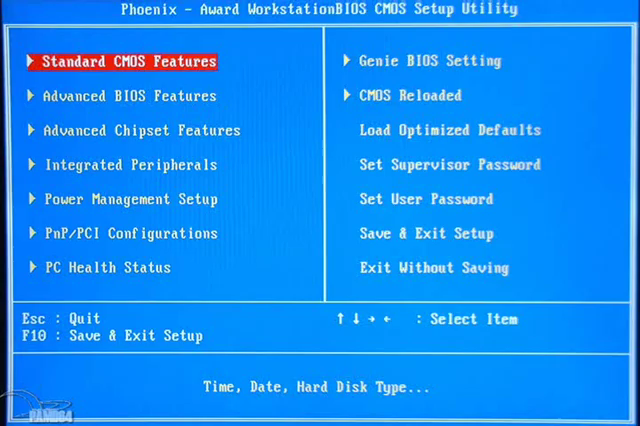
\includegraphics[scale=0.6]{img/00.png}
				\caption{La pantalla principal del CMOS Setup.}
			\end{figure}

		\subsubsection{Standard CMOS Setup}{\label{sub:Standard cmos setup}}
	
			``Standard CMOS Setup'' proviene del Ingles y significa literalmente:
			Configuración estándar de CMOS
			\begin{figure}[H]
				\centering
					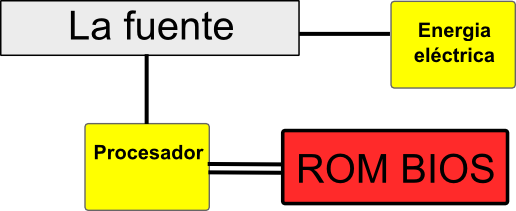
\includegraphics[scale=0.5]{img/01.png}
				\caption{La pantalla del ``Standard CMOS Setup''.}
			\end{figure}
			
			\begin{description}
				\item[Date] Asigna al sistema una fecha. El rango del mes es 1-12, del día 1-31 y del año 1994-2079.
				\item[Time] El formato es de 24 H, ejemplo la 1 de la tarde seria: 13: 00: 00.
				\item[Hard disk] {\emph Disco duro} - La BIOS soporta un
					DUAL-CHANNEL PIO y PCI BUS MASTER IDE. Cada puerto soporta
					una unidad maestra y otra esclava.

					{\large Explicación de las especificaciones de disco duro:}
                
					\begin{description}
						\item[Type] La BIOS contiene una tabla de tipos
							predefinidos. Si no coincide ninguna serie de
							valores, escoger USER.
						\item[Size] Capacidad aproximada del disco. Este tamaño
							suele ser ligeramente mayor que la capacidad una
							vez formateado el disco.
						\item[Cyls] Número de cilindros.
						\item[Head] Número de cabezas.
						\item[Precomp] Cilindro de precompensación de
							escritura. Este parámetro no tiene valor en los
							discos modernos.
					    \item[Landz] Zona de parada. Sólo para discos antiguos sin auto-aparcamiento.
					    \item[Sector] Número de sectores.
						\item[Mode] Auto, Normal, Large, o LBA\footnote{LBA
							(siglas de logical block addressing, dirección
							lógica de bloques) es un método muy común usado
							para especificar la localización de los bloques de
							datos en los sistemas de almacenamiento,
							principalmente secundario, del ordenador. El
							término LBA puede referirse también a la dirección
							del bloque al que enlaza.  Los bloques lógicos en
							los ordenadores modernos son normalmente de 512 o
							1024 bytes cada uno.}

						\begin{itemize}
							\item Auto: La BIOS detecta automáticamente el modo
								óptimo.  \item Normal: El número máximo de
								cilindros, cabezas y sectores soportado es
								1024, 16, y 63.
							\item Large: Discos que no soportan modo LBA y
								tienen más de 1024 cilindros. Solo unos pocos
								discos duros soportan este modo.
							\item LBA (Logical Block Addressrng): Durante los
								accesos a disco, la controladora IDE transforma
								la dirección de datos marcada por el número de
								sector, cabeza y cilindro en la dirección de
								bloque física, mejorando sensiblemente la tasa
								de transferencia de datos. Sólo para discos de
								más de 1024 cilindros.
						\end{itemize}
					\item[Floppy drives A \& B] Selecciona el tamaño de tu
						unidad de diskettes. Las opciones son: 360 KB (5.25”),
						720 KB (3.5”), 1.2 MB (5.25”), 1.44 MB (3.5”), 2.88 MB
						(3.5”).
					\item[Vídeo] Selecciona el tipo de adaptador de
						vídeo de tu PC. Estas son las posibilidades: EGA/VGA,
						MONO, CGA A 40 y CGA A 80.
					\item[Halt on] Durante el chequeo al encender el PC (POST),
						la BIOS se detiene si detecta algún error de hardware.
						Se puede indicar a la BIOS que ignore ciertos errores y
						continúe el proceso de arranque.

					\end{description}
				\end{description}

		\subsubsection{BIOS Features Setup}{\label{sub:bios features setup}}
			\begin{figure}[H]
				\centering
					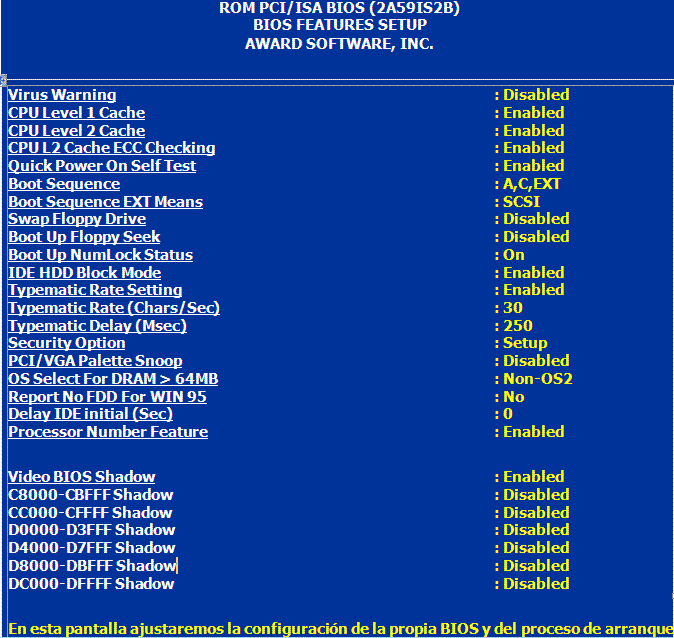
\includegraphics[scale=0.5]{img/02.png}
				\caption{``BIOS Features Setup''}
			\end{figure}
			
			\begin{description}
				\item[Virus Warning] Para impedir que algún soft borre el
					sector de arranque. Recomiendo DISABLE (Usar antivirus).
				\item[CPU Internal caché/External caché] Los datos almacenados
					en memoria caché se transfieren más rápidos, por ello ambas
					opciones deben estar ENABLED.
				\item[CPU L2 Caché ECC Checking] Si este parámetro está
					ENABLED, el procesador dota de un nivel extra de seguridad
					a los datos.
				\item[Quick Power On Self Test] ENABLED, reduce el tiempo
					necesario para realizar el chequeo de arranque (POST). Esto
					omite ciertos pasos. Es preferible que esté DISABLED.
				\item[Boot Sequence] Esta opción ordena, de entre varias
					opciones, la secuencia de arranque. Estas son las opciones
					disponibles: A, C, D, E, F, CD-ROM, SCSI y LS120 / ZIP.
				\item[Swap Floppy Drive] Asigna a la unidad A la letra B y
					viceversa, para ello deben estar las dos disqueteras
					ENABLED.
				\item[Boot Up Floppy Seek] Determina, si está ENABLED, si un
					diskette tiene 40 u 80 pistas. Sólo los diskettes de 360 KB
					tienen 40 pistas, por ello recomiendo DISABLED.
				\item[Boot Up Numlock Status] Activa o Desactiva la tecla Bloq
					Núm.
				\item[Boot Up System Speed] High, arranca a la velocidad por
					defecto del procesador, Low lo hace a la velocidad del BUS
					AT.
				\item[Gate A20 Option] La puerta A20 se refiere a como el
					sistema se comunica con la memoria por encima de 1MB
					(memoria extendida). Cuando se selecciona FAST, el chipset
					del sistema controla la puerta A20. Cuando se selecciona
					NORMAL, lo hace la controladora de teclado. Seleccionando
					FAST, la velocidad del sistema mejora, especialmente en
					OS/2 y Windows.
				\item[Typematic Rate Setting] DISABLED aplicaría los valores
					detallados más abajo y las teclas repetirían con frecuencia
					marcada por la controladora de teclado del sistema. Con
					ENABLED, se puede seleccionar el retraso y la frecuencia de
					repetición.
				\item[Typematic Rate (Chars/Sec)] Con ENABLED se selecciona el
					número de veces por segundo que se repite el caracter de
					una tecla pulsada.
				\item[Typematic Delay (Misc)] Con la opción Typematic Rate
					Setting ENABLED, podemos seleccionar el retraso en
					milisegundos hasta que una tecla pulsada empieza a repetir.
				\item[Security Option] Si se ha establecido una clave, debemos
					seleccionar si se pedirá cada vez que arranque el sistema
					(SYSTEM) o cuando se accede a la configuración (SETUP).
				\item[PCI/VGA Palette Snoop] Sólo se ha de dejar ENABLED si una
					tarjeta ISA instalada en el sistema lo requiriera, para
					sincronizar la tarjeta descompresora MPEG con la tarjeta
					gráfica o si se usa un convertidor VGA/TV.
				\item[OS Select from DRAM>64 MB] Se selecciona si el sistema
					operativo es OS/2 y el equipo tiene más de 64 Mbytes de
					memoria RAM.
				\item[Report No FDD For Win 95] Al seleccionar YES se libera la
					IRQ6 cuando el equipo no tiene disquetera (o no se quiere
					utilizar). Además, debemos deshabilitar el parámetro
					Onboard FDC Controller que podemos encontrar en el submenú
					INTEGRATED PHERIPHERALS de la BIOS.
				\item[Video BIOS Shadow] Pasa la ROM de la tarjeta de vídeo a
					memoria RAM; por lo tanto más rápida.
				\item[C8000 – CBFF/DC – DFFFF Shadow] Más especializado y
					concreto que Video BIOS Shadow, es preferible que esté
					DISABLED.
			\end{description}

		\subsubsection{Chipset Features Setup}{\label{sub:chipset features setup}}
			\begin{figure}[H]
				\centering
					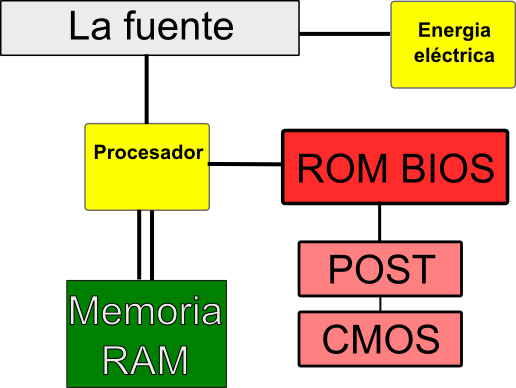
\includegraphics[scale=0.5]{img/03.png}
				\caption{``Chipset Features Setup''.}
			\end{figure}
			
			\begin{description}
				\item[Auto Configuration] Selecciona los valores óptimos
					predeterminados de la velocidad de memoria RAM para los
					parámetros del chipset (FX, HX, VX, TX) de la placa base.
					En caso de estar DISABLED, se vuelve a los valores
					almacenados cuando se instaló la placa base. Si se escoge
					ENABLED, ciertos valores de la sección no pueden
					modificarse. Para modificar estos valores y así obtener el
					máximo de prestaciones del equipo, se debe deshabilitar
					(DISABLED) la autoconfiguración. En algunos equipos no se
					puede deshabilitar.
				\item[EDO DRAM Speed Selection] El valor de este campo debe
					corresponder a la velocidad de la memoria RAM instalada en
					el equipo. NO cambiar los valores por defecto de este campo
					que han sido determinados por el fabricante de la placa
					para la RAM instalada. Este valor es la velocidad de
					acceso, por lo tanto un valor menor implica un equipo más
					rápido.
				\item[EDO CASx MA/RASx Wait State] Sólo para memoria EDO.
					Esto permite al fabricante insertar un estado de espera
					adicional para el refresco de las columnas de memoria. Para
					situar cada bit, el controlador de memoria debe fijar su
					dirección de columna (CAS) y su dirección en fila (RAS).
					Estos valores deben dejarse como están. Si se cambian y
					producen errores de memoria; debemos volver a los valores
					originales.
				\item[SDRAM RAS-to-CAS Delay] Este apartado permite insertar un
					ciclo de retraso entre las señales STROBE de CAS y RAS
					cuando se escribe, lee o refresca la memoria RAM.
				\item[SDRAM RAS Precharge Time] Si se establece tiempo
					insuficiente para que RAS acumule su carga antes del
					refresco de memoria RAM, el refresco puede ser incompleto y
					se pueden perder datos.
				\item[SDRAM CAS Latency Time] Cuando se instala memoria RAM
					síncrona (SDRAM), el número de ciclos de reloj de latencia
					CAS depende de la velocidad de memoria RAM. En general un
					valor menor aumenta las prestaciones y un valor mayor
					incrementa la estabilidad (Esto es aplicable para los tres
					últimos apartados).
				\item[SDRAM RAS Precharge Control] Si está ENABLED los ciclos
					de reloj refrescan todos los bancos de memoria. Estos
					cuatro últimos apartados sólo tienen valor cuando el
					sistema tiene instalada memoria SDRAM.
				\item[DRAM Data Integrity Mode] Selecciona el modo de
					corrección (paridad PARITY, o código de corrección de
					errores ECC) de acuerdo con el tipo de memoria RAM
					instalada.
				\item[System BIOS Cacheable] ENABLED permite copiar a la
					memoria caché la ROM BIOS del sistema en la dirección
					F0000h-FFFFFh, aumentando así las prestaciones. Sin
					embargo, si un programa escribe en este área se puede
					producir un error.
				\item[Video BIOS Cacheable] Permite copiar (ENABLED) a la
					memoria caché la ROM BIOS de la tarjeta gráfica aumentando
					las prestaciones.
				\item[Video RAM Cacheable] Aloja la caché de la tarjeta gráfica
					a la dirección A000 y B000 dentro de la memoria RAM; siendo
					así más rápida.
				\item[8/16 Bit I/O Recovery Time] Estos dos campos permiten
					añadir tiempo de recuperación (en ciclos de reloj del bus)
					para las órdenes de entrada y salida de los dispositivos
					ISA de 8 y 16 bits. En general, cuanto menor es el número
					mejores son las prestaciones, aunque deben hacerse pruebas
					con los valores seleccionados.
				\item[Memory Hole At 15M-16M] Se puede reservar este área de la
					memoria del sistema para la memoria ROM de las tarjetas
					ISA. Si se reserva, no se puede utilizar como caché. Ver el
					manual de los dispositivos por si lo necesitan.
				\item[Passive Relase] Esta función se utiliza para que puedan
					realizarse los accesos del procesador al bus ISA. Es
					recomendable habilitar o desahibilitar si se tienen
					problemas de compatibilidad con una tarjeta ISA.
				\item[Delayed Transaction] El chipset tiene un buffer de
					escritura de 32 bits para soportar ciclos retardados de
					transacciones. Selecciona ENABLED para que esté de acuerdo
					con la versión 2.1 del bus PCI. ENABLED mejora las
					prestaciones del equipo.
				\item[AGP Aperture SIZE (MB)] Selecciona el tamaño de apertura
					del Puerto de Gráficos Acelerados.  La apertura es una
					parte del rango de la dirección de memoria PCI dedicada
					para el espacio de dirección de la memoria gráfica.  El
					valor más habitual es 64MB, se estima que la cantidad
					idónea se obtiene igualando o dividiendo entre dos la
					memoria RAM instalada en el equipo.
				\item[CPU Host Clock] Por defecto viene en AUTO, pero podemos
					escoger las combinaciones: AUTO, 100, 103, 112 y 133 Mhz.
				    Estas son las frecuencias adecuadas que debemos combinar: \\ 

					\begin{tabular}{ l | c | c | c | r }
						\hline
	Frecuencia Ext. &      AGP         &    PCI    &    ISA    & DIMM \\ 
						\hline
	100 Mhz         &      66 Mhz      &  33 Mhz   &  8.33 Mhz & 100 Mhz \\ 
	103 Mhz         &     68.6 Mhz     & 34.3 Mhz  &  8.33 Mhz & 103 Mhz \\
	112 Mhz         &     74.6 Mhz     & 37.3 Mhz  &  8.33 Mhz & 112 Mhz \\ 
	133 Mhz         &    88.67 Mhz     & 44.33 Mhz &  8.33 Mhz & 133 Mhz \\ 
						\hline
					\end{tabular}
					
			\end{description}
			\newpage
			
		\subsubsection{Power Management Setup}{\label{sub:power management setup}}
			\begin{figure}[H]
				\centering
					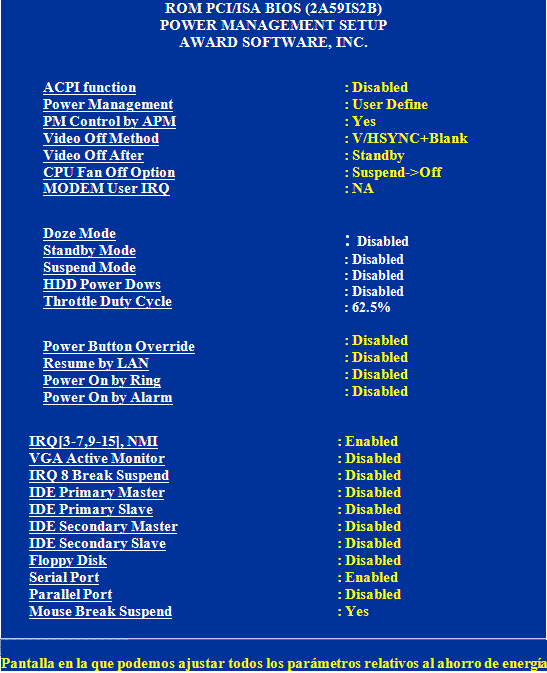
\includegraphics[scale=0.5]{img/04.png}
				\caption{``Power Management Setup''.}
			\end{figure}
				
			\begin{description}
				\item[Power Managament] Permite escoger el tipo o grado de
					ahorro de energía entre los modos Doze, Standby y Suspend.
					Esta tabla describe cada uno de los modos:

					\begin{tabular}{| l | r |}
						\hline
		 Max Saving  & Ahorro máximo. Sólo para procesadores SL (portátiles). \\ 
		 User Define & Establecer individualmente cada modo. \\ 
		 Min Saving  & Ahorro mínimo. \\ 
						\hline
					\end{tabular}
				\item[PM Control by APM] Seleccionando YES, el sistema avanzado
					de energía (APM), mejora el ahorro.
				\item[Video Off Method] Sistema para indicarle al monitor que
					debe entrar en un modo de ahorro de energía. Recomiendo:
					que sea consultado el manual del periférico para un ajuste
					optimo.  Estas son las opciones disponibles: DPMS OFF, DPMS
					reduce ON, Blank Screen, V/H SYNC+Blank, DPMS Standby, DPMS
					Suspend.
				\item[Video Off After] Esta opción permite que el monitor se
					adapte (se limpie) después de que el sistema haya entrado
					en Doze, Standby o Suspend mode. Se puede deshabilitar esta
					opción con el parámetro N/A. Por defecto el valor es
					Standby.
				\item[MODEM use IRQ / Wake up on LAN] Opciones que especifican
					la interrupción asignada al módem y si al detectar una
					llamada debe encenderse el sistema.
				\item[Doze Mode] Después del tiempo de inactividad
					seleccionado, el reloj del procesador va más lento aunque
					el resto de los componentes todavía operan a toda
					velocidad.
				\item[Standby Mode] Después del periodo de tiempo seleccionado,
					el disco duro y la tarjeta gráfica se apagan mientras que
					los otros dispositivos siguen funcionando.
				\item[Suspend Mode] Después del periodo de inactividad
					seleccionado, todos los dispositivos excepto el procesador
					se apagan.
				\item[HDD Power Down] Después del tiempo seleccionado de
					inactividad, el disco duro se apaga pero los otros
					dispositivos no.
				\item[Throttle Duty Cycle] Cuando el sistema entre en modo
					Doze, el reloj del procesador corre sólo parte del tiempo.
					Aquí se puede seleccionar el porcentaje de ese equipo.
				\item[PCI/VGA Act-Monitor] Habilita o deshabilita la detección
					de inactividad del monitor.
				\item[Soft-Off by PWR-BTTN] Pone al equipo en un modo de muy
					bajo consumo, Instand-off hace que vuelva inmediatamente a
					estar disponible al tocar el botón ON/OFF o recibir una
					llamada por el módem. Con Delay 4 Sec., el sistema espera 4
					segundos antes de hacer todo lo anterior.
				\item[CPUFAN off In Suspend] El ventilador del procesador se
					apagará cuando este esté inactivo.  Resume by Ring: Una
					llamada al módem anula el modo de ahorro de energía.
				\item[Resume by Alarm / Date (of Month) Alarm, Time (hh:mm:ss)
					Alarm] Con el primer parámetro habilitamos o deshabilitamos
					al segundo, que permite establecer la fecha y hora para que
					el equipo despierte del modo suspendido.
				\item[IRQ 8 Break Suspend] Se puede habilitar o deshabilitar la
					monitorización de la IRQ8 (Real Time Clock, Reloj en tiempo
					real) para que no anule el modo Suspend de ahorro de
					energía.
				\item[Reload Global Timer Events] Cuando está ENABLED cualquier
					operación de los dispositivos listados reinicia el
					temporizador para el modo Standby.
			\end{description}
			\newpage
		\subsubsection{PNP/PCI Configuration}{\label{sub:pnp/pci configuration}}
			\begin{figure}[H]
				\centering
					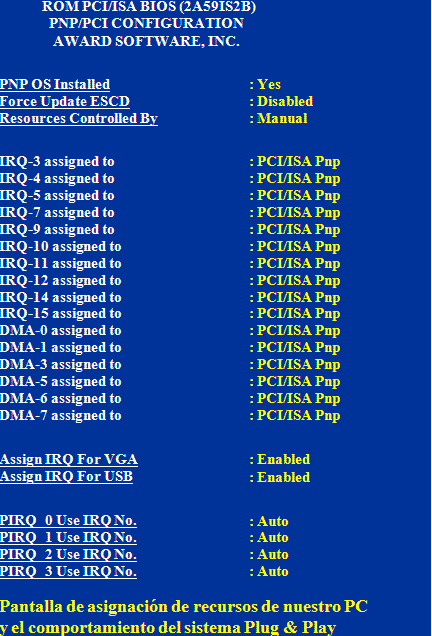
\includegraphics[scale=0.5]{img/05.png}
				\caption{``Configuracion de PNP/PCI''.}
			\end{figure}
			\begin{description}
				\item[PNP OS Instaled] Activar siempre que se haya instalado un
					sistema operativo PnP. Recomiendo activarla para Windows 95
					o posteriores.
				\item[Resources Controlled By] La BIOS de tipo Plug and Play
					configura automáticamente los dispositivos que cumplen
					dicho estándar. Si se selecciona AUTO, desaparecen los
					campos IRQ y DMA, porque la BIOS los asigna
					automáticamente.
				\item[Reset Configuration Data] Normalmente este valor está
					DISABLED. Se selecciona ENABLED para reiniciar los datos de
					configuración al salir de la BIOS, después de haber
					instalado un dispositivo o haber cambiado valores debido a
					un fallo en el encendido del equipo.
				\item[IRQ-xx assigned to / DMA-x assigned to] Estos parámetros
					reservan IRQ (petición de interrupción) o canales DMA
					(acceso directo a memoria) a ciertos dispositivos. Si
					tenemos una tarjeta ISA y esta no es PnP, requiere una
					interrupción IRQ o un canal DMA que soporten esa función,
					para ello debemos asignar a los susodichos IRQ o DMA la
					opción “Legacy ISA”.
				\item[Used MEM base addr] Este parámetro, en conjunción con
					“Used MEM Length” asignan la dirección base para el área de
					memoria usada por cualquier periférico que requiera memoria
					alta (de 640 KB a 1 MB).
				\item[Assign IRQ For USB] Por defecto viene ENABLED. Se puede
					Deshabilitar si necesitamos alguna IRQ extra y carecemos de
					dispositivos USB que las ocupen.
			\end{description}

		\newpage

	\subsection{Restaurar la configuración del CMOS Setup}{\label{sec:cmossetup/resetear-el-cmos-setup}}

		Hay varias formas de restaurar la configuración del CMOS Setup o bien del chip CMOS. \\
		Generalmente no se lo hace, pero en caso de olvidar la contraseña de acceso

	\subsubsection{Batería CMOS}{\label{sec:bateria cmos}}

		Sacar la pila del CMOS que se encuentra sujetada en un slot para la pila en
		la placa base por unos segundos, despues reemplazarla otravez.

	\subsubsection{El RESET CMOS}\label{sec:el reset cmos}

	\begin{figure}[H]
		\centering
			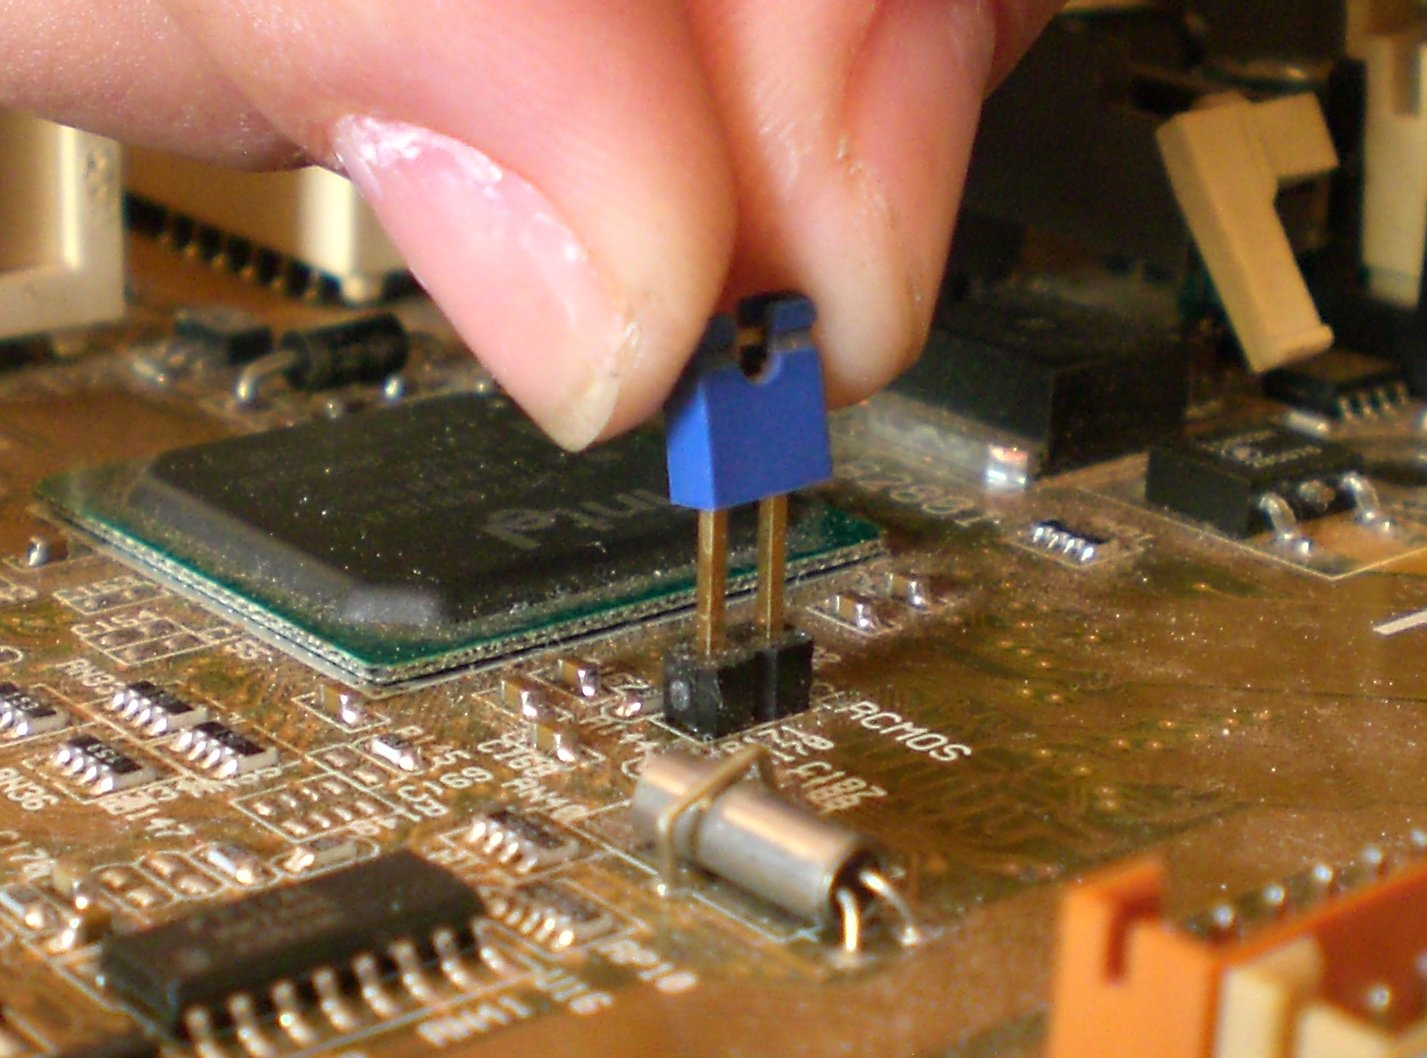
\includegraphics[scale=0.2]{img/RESET_CMOS.JPG}
		\caption{El ``RESET CMOS''}
	\end{figure}
	Algunas placas base ofrecen un jumper CMOS-reset o un botón de reinicio.

	\subsubsection{Metodo programativo}\label{sec:metodo programativo}

	En otros casos, el chip EEPROM ha de desoldar los datos en forma manual,
	por manos de un programador. 
	A veces es suficiente motivo para el CLK o línea de DTA de la I2C bus de la
	EEPROM en el momento adecuado durante el arranque, esto requiere una cierta
	precisión en las piezas de soldadura SMD. 
	Si la máquina le permite arrancar, pero no quiere que le permiten a la
	configuración de la BIOS, una posible recuperación es dañar la suma de
	comprobación CMOS, haciendo puerto directo escribe usando debug.exe,
	corrompiendo a algunos bytes de la suma de control de área protegida de la
	RAM CMOS, en el siguiente arranque, el equipo normalmente restablece su
	configuración de fábrica. Por ejemplo:

	\begin{verbatim}
	c:\debug
	-o 70 10
	-o 71 aa
	-q
	\end{verbatim}

	Que permitirá escribir en CMOS (Offset 10h) con el valor 0AAhA.

	\newpage

\appendix

\section{Anexo}\label{sec:anexo}
	\subsection{POST}\label{sub:post}
	
		El POST es el acrónimo inglés de Power On Self Test (Auto diagnóstico
		al encender). Es un proceso de verificación e inicialización de los
		componentes de entrada y salida en un sistema de cómputo que se encarga
		de configurar y diagnosticar el estado del hardware.

	\subsection{CPU Cache}\label{sub:cpu cache}
	
		A CPU cache is a cache used by the central processing unit of a
		computer to reduce the average time to access memory. The cache is a
		smaller, faster memory which stores copies of the data from the most
		frequently used main memory locations. As long as most memory accesses
		are cached memory locations, the average latency of memory accesses
		will be closer to the cache latency than to the latency of main memory.
		When the processor needs to read from or write to a location in main
		memory, it first checks whether a copy of that data is in the cache. If
		so, the processor immediately reads from or writes to the cache, which
		is much faster than reading from or writing to main memory.  Most
		modern desktop and server CPUs have at least three independent caches:
		an instruction cache to speed up executable instruction fetch, a data
		cache to speed up data fetch and store, and a translation lookaside
		buffer used to speed up virtual-to-physical address translation for
		both executable instructions and data.



	\subsection{IEEE 1284 (LPT)}\label{sub:ieee 1284 (lpt)}
		
		El estándar IEEE 1284 (Standard Signaling Method for a {\emph Bi-directional
		Parallel Peripheral Interface for Personal Computers}, en español,
		Estándar del Método de Señalización para una Interfaz Paralela
		Bidireccional Periférica para Computadoras Personales), aprobado para
		su publicación en marzo de 1994, provee de una comunicación de alta
		velocidad y bidireccional entre un ordenador y un dispositivo externo
		que puede comunicarse 50 ó 100 veces más rápido que con el puerto
		paralelo original; además de ser totalmente compatible con los
		periféricos, impresoras y software que existían previamente.

		\cite{LPT}

	\subsection{Plug-and-Play}\label{sub:plug-and-play}
	
		Plug-and-play (conocida también por su abreviatura PnP) es la
		tecnología que permite a un dispositivo informático ser conectado a un
		ordenador sin tener que configurar (mediante jumpers o software
		específico (no controladores) proporcionado por el fabricante) ni
		proporcionar parámetros a sus controladores. Para que sea posible, el
		sistema operativo con el que funciona el ordenador debe tener soporte
		para dicho dispositivo.

		\cite{plugandplay}

\newpage

\clearpage
\section{Bibliografía}
\begin{thebibliography}{99}\label{sec:bibliografia}

	\bibitem{WIC}
		What is CMOS?,
		\url{http://www.wisegeek.com/what-is-cmos.htm}

	\bibitem{UnidadIIBIOSExposicion.ppt}
		% CORREGIR!
		Exposicion de BIOS de la Universidad BLABLA

	\bibitem{BIOS01}
		``BIOS'' - {\em Basic Input-Output System}
		\url{http://es.wikipedia.org/wiki/BIOS}

	\bibitem{BIOS02}
		Monografias - {\em ``BIOS''}
		\url{http://www.monografias.com/trabajos37/la-bios/la-bios.shtml}

	\bibitem{CIL}
		Dan Clein, ``CMOS IC LAYOUT Concepts, Methodologies, and Tools'', pp. 22 - 26, 2000

	\bibitem{MDB}
		Mesmer, ``Manual de la BIOS'', Marzo 2001
	
	\bibitem{BootProcess}
		\url{http://duartes.org/gustavo/blog/post/how-computers-boot-up/}
	
	\bibitem{BootSequence}
		\url{http://www.pcguide.com/ref/mbsys/bios/bootSequence-c.html}

	\bibitem{EEPROM}
		{\em Memory EEPROM}
		\url{http://es.wikipedia.org/wiki/EEPROM}
	
	\bibitem{LPT}
		Wikipedia - ``LPT''
		\url{http://es.wikipedia.org/wiki/LPT}

	\bibitem{plugandplay}
		Wikipedia - ``Plug-and-play''
		\url{http://es.wikipedia.org/wiki/Plug-and-play}

\end{thebibliography}


\end{document}
